
\documentclass{beamer} 
\usetheme{Boadilla}
\usecolortheme{beaver}

\usepackage[utf8]{inputenc}
\usepackage[portuguese]{babel}
\usepackage{lmodern}
\usepackage[absolute,overlay]{textpos}
\usepackage{verbatim}
\newenvironment{reference}[2]{% 
  \begin{textblock*}{\textwidth}(#1,#2) 
      \footnotesize\it\bgroup\color{red!50!black}}{\egroup\end{textblock*}} 
\title{Defesa de sistemas de informação}
\author[Lopez. V.L.O, Winck. A. T]{Víctor Orozco, Dr. Ana Trindade Winck}
\institute[UFSM]{
  Centro de Tecnologia \\
  Universidade Federal de Santa Maria
}
\date{\today}

\begin{document}
\begin{frame}[Plain]
\titlepage
\end{frame}

\begin{frame}{Objetivos da aula}
\begin{itemize}
\item Descrever mecanismos generalizados de defesa de sistemas
\item Apresentar uma definição conceptual de controles de segurança
\item Apresentar uma classificação de controles de segurança
\end{itemize}
\end{frame}

\begin{frame}
\frametitle{Roteiro}
\tableofcontents
\end{frame}

\section{Defesa de sistemas de informação}
\begin{frame}{Defesa de sistemas de informação}
\begin{figure}[tbph]
\centering
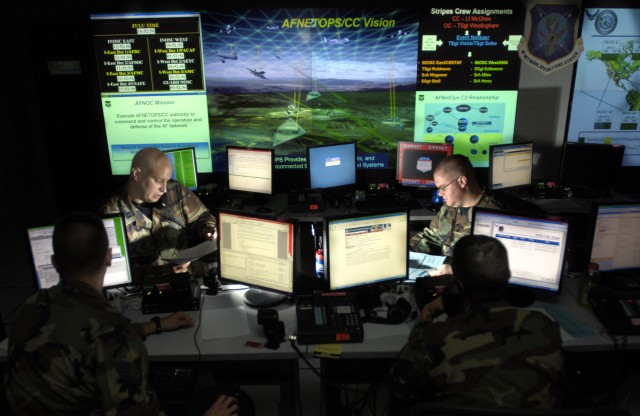
\includegraphics[width=0.7\linewidth]{./CyberCommand}
\label{fig:CyberCommand}
\end{figure}
\end{frame}

\begin{frame}{Defesa}
\begin{figure}[tbph]
\centering
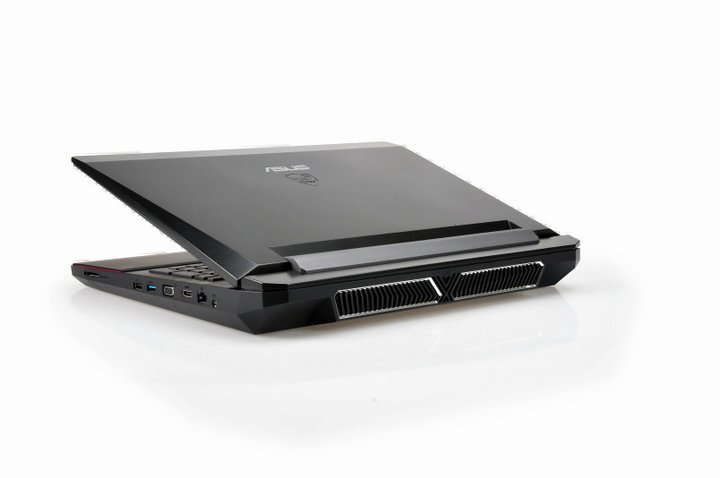
\includegraphics[width=0.7\linewidth]{./laptop}
\label{fig:laptop}
\end{figure}
\end{frame}

\begin{frame}{Preciso defender?}
\begin{figure}[tbph]
\centering

\includegraphics[width=0.3\linewidth]{./question}
\label{fig:question}
\end{figure}
\end{frame}

\begin{frame}{Preciso defender?}
Depende
\end{frame}

\begin{frame}{Defesa}
\begin{itemize}
\item Ativos 1-10
\item Importância+impacto
\end{itemize}
\end{frame}

\begin{frame}{Defesa}
\begin{itemize}
\item Fotos da família - 2
\item Filmes - 1
\item Jogos (NFS nivel 10) - 1
\item Coleção musicas (250gb) - 5
\end{itemize}
\end{frame}

\begin{frame}{Defesa}
\begin{itemize}
\item Dissertação de mestrado - 7
\item Artigos en andamento - 9
\item Documentação para renovação de visto de estudante - 10
\item Arquivos de personalização do meu sistema operacional - 9
\end{itemize}
\end{frame}

\begin{frame}{Defesa}
Vale muito a pena
\end{frame}

\begin{frame}{Defesa}
\begin{figure}[tbph]
\centering

\includegraphics[width=0.3\linewidth]{./question}
\label{fig:question2}
\end{figure}
\end{frame}

\begin{frame}{Defesa}
\begin{itemize}
\item Timeout de atividade
\item Password BIOS
\item Password sistema operacional
\item Criptografia de HD em dados importantes
\item Monitoramento remoto (Prey)
\item Firewall
\item Backup on-site semanal
\item Backup na nuvem de documentos en andamento
\item Atualizações semanais
\item Boletim de segurança do Gentoo Linux
\item Keyring de senhas
\end{itemize}
\end{frame}

\begin{frame}{Defesa}
Investimento: \$ 100 (HD externo)
\end{frame}

\begin{frame}{Defesa (experiencias)}
\begin{itemize}
\item Um pendrive com um vírus 0day estragou meu Windows um dia antes da entrega duma tarefa
\item Foi roubado um pendrive com todos os endereços de email da minha faculdade
\item Uma versão desatualizada do Joomla deu controle para hackers Islamicos - não é piada
\end{itemize}
\end{frame}

\begin{frame}{Defesa em profundidade}
\begin{itemize}
\item Estrategia muito conhecida e comum
\item Formular uma defesa de várias camadas que nos permitirá ainda montar um sucesso se uma ou mais de nossas medidas defensivas apresentam falhas
\end{itemize}
\end{frame}

\begin{frame}{Defesa em profundidade}
\begin{figure}[tbph]
\centering
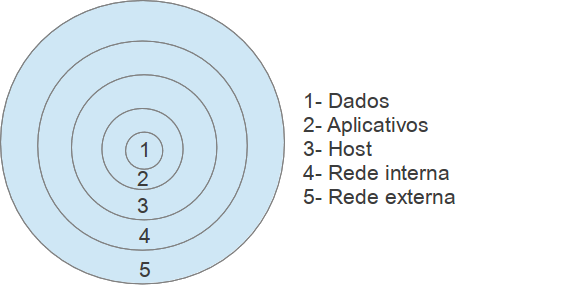
\includegraphics[width=0.7\linewidth]{./capas}
\label{fig:capas}
\end{figure}
\end{frame}

\begin{frame}{Defesa em profundidade}
\begin{itemize}
\item Ela não é uma bala magica
\item Não vamos ser capazes de manter todos os atacantes fora por um período indefinido de tempo
\item Colocar suficientes medidas defensivas entre nossos ativos é os atacantes
\item Comprar tempo suficiente para tomar medidas mais efetivas para impedir o ataque.
\end{itemize}
\end{frame}

\section{Controles de segurança}
\begin{frame}{Controles de segurança}
\begin{itemize}
\item Medidas para ajudar a garantir que um determinado tipo de ameaça é contabilizada (neutralizada, prevenida)
\item Físicos
\item Lógicos
\item Administrativos
\end{itemize}
\end{frame}


\begin{frame}{Fisicos}
\begin{itemize}
\item Controles do lugar onde nossos sistemas e/ou a nossa informação foi guardada.
\item Acesso ?
\item Manter o meio físico ?
\end{itemize}
\end{frame}

\begin{frame}{Fisicos}
\begin{itemize}
\item Controles do lugar onde nossos sistemas e/ou a nossa informação foi guardada.
\item Acesso: Cercas, portões, fechaduras.
\item Manter o meio físico: sistemas de ar condicionado, sistemas de extinção de incêndio e geradores de energia.
\end{itemize}
\end{frame}

\begin{frame}{Fisicos}
\begin{itemize}
\item Se não formos capazes de proteger fisicamente os nossos sistemas e dados, quaisquer outros controles são irrelevantes.
\item Se um atacante tem acesso físico pode acontecer:
\begin{itemize}
\item Melhor caso: Destruir a nossa informação
\item Pior caso: Roubar a nossa informação e fazer com ela o que quiser
\end{itemize}
\end{itemize}
\end{frame}

\begin{frame}{Logicos}
\begin{itemize}
\item Também chamados de controles técnicos, protegem o ambiente que trafega e armazena os nossos dados
\item Acesso ?
\item Detecção ?
\end{itemize}
\end{frame}

\begin{frame}{Logicos}
\begin{itemize}
\item Também chamados de controles técnicos, protegem o ambiente que trafega e armazena os nossos dados.
\item Acesso: Passwords, criptografia, firewalls
\item Detecção: Antivírus, antispyware, sistemas de detecção de intrusão 
\end{itemize}
\end{frame}

\begin{frame}{Logicos}
\begin{itemize}
\item Se nossos controles lógicos são implementadas adequadamente e são sucesso, um atacante ou usuário não autorizado não pode acessar nossas aplicações e dados sem subverter os controles que temos no lugar.
\item Melhor caso: O acesso foi vulnerado mas foi detectado a tempo
\item Pior caso: As medidas falharam e o atacante tem liberdade
\end{itemize}
\end{frame}

\begin{frame}{Administrativos}
\begin{itemize}
\item Definem as regras do comportamento esperado dos nossos usuários e o meio ambiente
\item Papel ?
\item Monitoramento ?
\end{itemize}
\end{frame}

\begin{frame}{Administrativos}
\begin{itemize}
\item Definem as regras do comportamento esperado dos nossos usuários e o meio ambiente
\item Papel: Regras, leis, políticas, procedimentos, diretrizes
\item Monitoramento: Capacidade de forçar as regras
\end{itemize}
\end{frame}

\begin{frame}{Administrativos}
\begin{itemize}
\item Se não temos a autoridade ou a capacidade de garantir que nossos controles estão sendo cumpridos, eles criam uma falsa sensação de segurança.
\item Uso de telefone e celular, acesso à Web, e-mail, uso conversas de mensagens instantâneas, o software instalado, e outras áreas potenciais de abuso.
\end{itemize}
\end{frame}

\begin{frame}{Defesa em profundidade}
\begin{figure}[tbph]
\centering
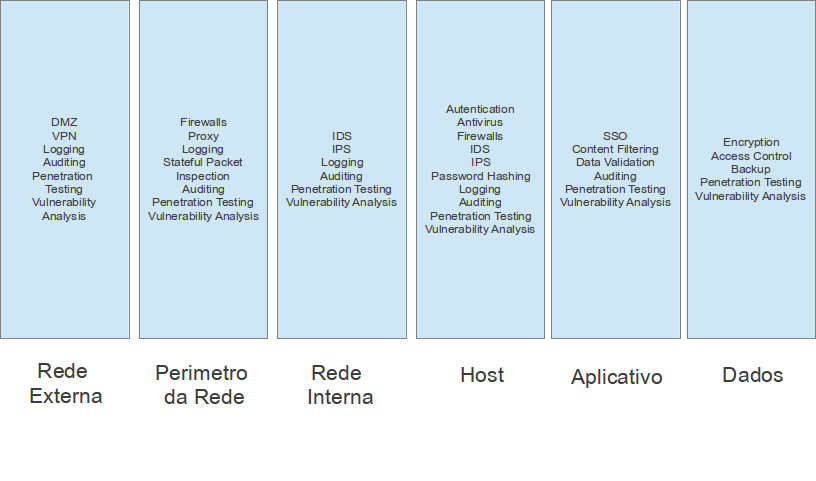
\includegraphics[width=0.9\linewidth]{./capasimp.png}
\label{fig:capasimp}
\end{figure}
\end{frame}

\section{Referencias}
\begin{frame}[allowframebreaks]{Referencias}
    \bibliographystyle{sbc}
    \bibliography{small}
\end{frame}
\end{document}